\ifx\wholebook\relax \else

\documentclass[UTF8]{article}
\usepackage[nomarginpar
  %, margin=.5in
]{geometry}

\addtolength{\oddsidemargin}{-0.05in}
\addtolength{\evensidemargin}{-0.05in}
\addtolength{\textwidth}{0.1in}

\usepackage[cn]{../../prelude}

\setcounter{page}{1}

\begin{document}

\title{Preface}

\author{Liu Xinyu
\thanks{{\bfseries Liu Xinyu} \newline
  Email: liuxinyu95@gmail.com \newline}
  }

\maketitle
\fi

\markboth{Preface}{Mathematics of Programming}

\chapter*{Preface}
%\phantomsection  % so hyperref creates bookmarks
%\addcontentsline{toc}{chapter}{Preface}

Martin Gardner gives an interesting story in his popular book {\em aha! Insight}. In a country fair, there is a game called ``Fifteen'' on the carnival midway. Mr. Carny, the carnival operator explained people the rules: ``We just take turns putting down coins on a line of numbers from 1 to 9. It doesn't matter who goes first. You put on nickles, I put on silver dollars. Whoever is the first to cover three different numbers that add to 15 gets all money on the table.''

\vspace{5mm}
\begin{tabular}{|c|c|c|c|c|c|c|c|c|}
\hline
1 & 2 & 3 & 4 & 5 & 6 & 7 & 8 & 9 \\
\hline
\end{tabular}
\vspace{5mm}

A lady joined this game. She went first by putting a nickle on 7. Because 7 was covered, it couldn't covered again by either player. And it's the same for other numbers. Mr. Carny then put a dollar on 8.

\vspace{5mm}
\begin{tabular}{|c|c|c|c|c|c|c|c|c|}
\hline
1 & 2 & 3 & 4 & 5 & 6 & 7 & 8 & 9 \\
\hline
  &   &   &   &   &   & nickle & dollar & \\
\hline
\end{tabular}
\vspace{5mm}

The lady next put a nickle on 2, so that one more nickle on 6 would make 15 and win the game for her. But the man blocked her with a dollar on 6. Now he could win by covering 1 on his next turn.

\vspace{5mm}
\begin{tabular}{|c|c|c|c|c|c|c|c|c|}
\hline
1 & 2 & 3 & 4 & 5 & 6 & 7 & 8 & 9 \\
\hline
  & nickle  &   &   &   & dollar  & nickle & dollar & \\
\hline
\end{tabular}
\vspace{5mm}

Seeing this threat, the lady put a nickle on 1 to block his win.

\vspace{5mm}
\begin{tabular}{|c|c|c|c|c|c|c|c|c|}
\hline
1 & 2 & 3 & 4 & 5 & 6 & 7 & 8 & 9 \\
\hline
nickle  & nickle  &   &   &   & dollar & nickle & dollar & \\
\hline
\end{tabular}
\vspace{5mm}

The carnival man then put a dollar on 4. He would win by covering 5 next. The lady had to block him again. She put a nickle on 5.

\vspace{5mm}
\begin{tabular}{|c|c|c|c|c|c|c|c|c|}
\hline
1 & 2 & 3 & 4 & 5 & 6 & 7 & 8 & 9 \\
\hline
nickle  & nickle  &   & dollar  & nickle  & dollar  & nickle & dollar & \\
\hline
\end{tabular}
\vspace{5mm}

But the carnival man placed a dollar on 3. He won because 3 + 4 + 8 = 15. The poor lady lost all nickles.

\vspace{5mm}
\begin{tabular}{|c|c|c|c|c|c|c|c|c|}
\hline
1 & 2 & 3 & 4 & 5 & 6 & 7 & 8 & 9 \\
\hline
nickle  & nickle  & dollar  & dollar  & nickle  & dollar  & nickle & dollar & \\
\hline
\end{tabular}
\vspace{5mm}

Many people joined to play the game. The town's Mayor was fascinated by the game, too. After watching it for a long time, he decided that the carnival man had a secrete that made him never to lose the game except he wanted to. The Mayer was awake all night trying to figure out he secrete.

There was a legend about Luo Shu in ancient China back to the time of huge flood. A turtle emerged from the river with a curious pattern on its shell: a 3 $\times$ 3 grid in which circular dots of numbers were arranged.

\begin{figure}[htbp]
 \centering
 \subcaptionbox{Luo Shu Square}[0.45\linewidth]{ 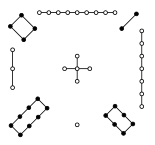
\includegraphics[scale=0.6]{img/luo-shu.png}}
 \subcaptionbox{Magic square of order 3}[0.45\linewidth]{
   \begin{tabular}{|c|c|c|}
   \hline
   4 & 9 & 2 \\
   \hline
   3 & 5 & 7 \\
   \hline
   8 & 1 & 6 \\
   \hline
   \end{tabular}
   \vspace{8mm}
 }
 \captionsetup{labelformat=empty}
 \caption{}
 \label{fig:luo-shu}
\end{figure}

% 考虑一一映射反向的情况。
This is known as Luo Shu Square, a magic square of order 3. The sum of the numbers in each row, column and diagonal was the same: 15. For example:

可别被这个名字吓到,就是方形的九个格子里每行、每列、两个对角线上的三个数字加起来都相等,都等于十五。例如第一行的数字相加是4 + 9 + 2 = 15,第三列的数字相加是2 + 7 + 6 = 15,左上右下的对角线的数字相加是4 + 5 + 6 = 15。等一等——马爷爷想,我现在知道庙会里套圈游戏背后的秘密了。如果要套中的三个玩具加起来等于十五元,那么就相当于套中了幻方的一行、一列、或一个对角线。如果摊主在柜台里偷偷藏一张三阶幻方的图,那么他实际上相当于在和游人玩俗称“一条龙”的井字棋游戏。

\begin{figure}[htbp]
 \centering
 \subcaptionbox{三阶幻方}[0.45\linewidth]{
   \begin{tabular}{|c|c|c|}
   \hline
   4 & 9 & 2 \\
   \hline
   3 & 5 & 7 \\
   \hline
   8 & 1 & 6 \\
   \hline
   \end{tabular}
   \vspace{3mm}
 }
 \subcaptionbox{井字棋游戏}[0.45\linewidth]{
   \begin{tabular}{c|c|c}
   $\times$ &  & $\bigcirc$ \\
   \hline
   $\times$ & $\times$ &  \\
   \hline
   $\bigcirc$ & $\times$ & $\bigcirc$ \\
   \end{tabular}
   \vspace{3mm}
 }
 \captionsetup{labelformat=empty}
 \caption{}
 \label{fig:bingo-magic-square}
\end{figure}

庙会中那个小男孩和摊主的套圈游戏相当于下面的井字棋对局。摊主在关键的第三步中给小男孩设置了一个陷阱,他在第一列上和一个对角线上同时可能连成直线,如果小男孩套中3,则摊主套中5依然能赢。如果了解过博弈游戏,或者知道一点编程,你就知道井字棋游戏没有必胜的策略,如果游戏双方都足够小心,结果一定是平局。偷偷拥有三阶幻方图的摊主这样就站在了不败的地位上,而其他游客一无所知。

\begin{figure}[htbp]
 \centering
 \subcaptionbox{三阶幻方}[0.45\linewidth]{
   \begin{tabular}{|c|c|c|}
   \hline
   4 & 9 & 2 \\
   \hline
   3 & 5 & 7 \\
   \hline
   8 & 1 & 6 \\
   \hline
   \end{tabular}
   \vspace{3mm}
 }
 \subcaptionbox{第一步,男孩套中7,摊主套中8}[0.45\linewidth]{
   \begin{tabular}{c|c|c}
   &  & \\
   \hline
   &  & $\times$ \\
   \hline
   $\bigcirc$ & & \\
   \end{tabular}
   \vspace{3mm}
 } \vspace{3mm} \\
 \subcaptionbox{第二步,男孩套中2,摊主套中6}[0.45\linewidth]{
   \begin{tabular}{c|c|c}
   &  & $\times$\\
   \hline
   &  & $\times$ \\
   \hline
   $\bigcirc$ & & $\bigcirc$ \\
   \end{tabular}
   \vspace{3mm}
 }
 \subcaptionbox{第三步,男孩套中1,摊主套中4}[0.45\linewidth]{
   \begin{tabular}{c|c|c}
   $\bigcirc$ &  & $\times$\\
   \hline
   &  & $\times$ \\
   \hline
   $\bigcirc$ & $\times$ & $\bigcirc$ \\
   \end{tabular}
   \vspace{3mm}
 } \vspace{3mm} \\
 \subcaptionbox{第四步,男孩套中5,摊主套中3,摊主胜}[0.45\linewidth]{
   \begin{tabular}{c|c|c}
   $\pmb{\bigcirc}$ &  & $\times$\\
   \hline
   $\pmb{\bigcirc}$ &  $\times$ & $\times$ \\
   \hline
   $\pmb{\bigcirc}$ & $\times$ & $\bigcirc$ \\
   \end{tabular}
   \vspace{3mm}
 }
 \captionsetup{labelformat=empty}
 \caption{}
 \label{fig:game-steps}
\end{figure}

这个故事是真的么?当然不是,马爷爷是个虚构的人物,他在真实世界中名叫马丁$\cdot$加德纳——举世闻名的美国趣味数学大师。这个故事来自他的《啊哈!灵机一动》。故事不是发生在北京的地坛公园,而是美国的乡村小镇。摊主名叫卡内,而玩游戏的小男孩实际是一位女士。这个游戏也不是中国传统的套圈游戏,而是用硬币盖住一排数字。

这个故事和其中所讲的游戏不断在说着一个重要的概念——同构。一行九个数字和三行三列的格子同构,相加等于15的目标与行、列、对角线同构,古老的《洛书》和数学幻方同构,马爷爷和加德纳同构,中国的春节庙会和美国乡村游乐同构……这其实也是本书想传达的概念,编程和数学同构,和艺术同构,和音乐同构。伟大的发现背后有曲折的故事和性格迥异的数学家。

这个故事还有一层隐喻,问题的表象下隐藏着和它同构的理论实质,我们需要了解抽象的本质而不被具体的现象蒙住眼睛。在人工智能和机器学习日新月异的今天,我们能否还靠着一点点聪明和工程实践继续前行?我们是否要打开那些神秘的黑盒子找到那个指引我们前进的地图?

\vspace{15mm}

刘新宇

二零一九年五月于北京

\begin{Exercise}
\Question{编程实现一个井字棋游戏是传统人工智能中的经典问题,而计算机可以轻松算出三个数字的和并判断其是否等于15。请利用这个同构编写一个简化的井字棋程序,并做到不被人类玩家击败。}
\end{Exercise}

\vspace{10mm}

本书的电子版可以在\url{https://github.com/liuxinyu95/unplugged}下载。如果希望获得纸质版,请联系作者:liuxinyu95@gmail.com

\ifx\wholebook\relax \else

\expandafter\enddocument
%\end{document}

\fi
